% Keep the supplied class unchanged. pdfLaTeX uses its original spot colours.
% Tectonic/XeTeX preview uses the identical declared CMYK colour because the
% template's 2006 spotcolor package only implements pdfTeX primitives.
\RequirePackage{iftex}
\ifXeTeX
  \RequirePackage[T1]{fontenc}
  \RequirePackage{color}
  \makeatletter
  \@namedef{ver@spotcolor.sty}{2026/09/16 XeTeX preview compatibility}
  \newcommand\NewSpotColorSpace[1]{}
  \newcommand\AddSpotColor[4]{}
  \newcommand\SetPageColorSpace[1]{}
  \def\color@spotcolor#1#2{\color@cmyk#1{1,0.3,0,0.2}}
  \makeatother
\fi

\documentclass[nolineno]{ieeeaccess}
\usepackage{cite}
\usepackage{amsmath,amssymb,amsfonts}
\usepackage{graphicx}
\usepackage{booktabs}
\usepackage{tabularx}
\usepackage{textcomp}
\usepackage{xurl}
\usepackage[hidelinks]{hyperref}
\usepackage{iftex}
\usepackage{etoolbox}
\usepackage{needspace}
\usepackage{placeins}
% Explicit aliases for two shapes requested by the supplied class.
\makeatletter
\InputIfFileExists{t1pcr.fd}{}{}
\DeclareFontShape{T1}{pcr}{n}{n}{<->ssub*pcr/m/n}{}
\DeclareFontShape{T1}{formata}{m}{sl}{<->ssub*formata/m/it}{}
\makeatother
\patchcmd{\IEEEbiographynophoto}{\vskip 4\baselineskip plus 1fil minus 0\baselineskip}{\vskip 2\baselineskip}{}{}
% Retain the venue's layout without inheriting its sample volume/year.
\makeatletter
\newcommand{\draftfooter}{\hbox to\textwidth{\footervolfont AUTHOR-REVIEW DRAFT -- SEPTEMBER 2026\hfill\footerpagefont\thepage}}
\apptocmd{\ps@titlepage}{\let\@oddfoot\draftfooter\let\@evenfoot\draftfooter}{}{}
\apptocmd{\ps@headings}{\let\@oddfoot\draftfooter\let\@evenfoot\draftfooter}{}{}
\makeatother
% The supplied class's Type-1 fonts also work with Tectonic/XeTeX.
\ifXeTeX
\special{pdf:mapfile t1-times.map}
\special{pdf:mapfile t1-formata.map}
\special{pdf:mapfile t1-giovannistd.map}
\fi
\graphicspath{{figures/}}
% The supplied class aliases these lengths; allocate a separate abstract box
% so its bullet and inset fit inside the title width without an overfull box.
\newlength{\paperabstractwidth}
\setlength{\paperabstractwidth}{\dimexpr\titlewidth-10pt\relax}
\let\abstractwidth\paperabstractwidth
\setcounter{dbltopnumber}{3}
\renewcommand{\dbltopfraction}{.9}
\renewcommand{\topfraction}{.9}
\renewcommand{\textfraction}{.08}
\hypersetup{pdftitle={Evaluating Vision-Based Tyre Inspection: Checkpoint Sensitivity, Region Interventions, and Boundary Localisation},pdfauthor={Sreenivasa Reddy Edara, Shanmukesh Bonala}}
\begin{document}
\raggedbottom
\pagestyle{headings}
\history{Author-review manuscript, September 18, 2026.}
\doi{Not assigned}
\title{Evaluating Vision-Based Tyre Inspection: Checkpoint Sensitivity, Region Interventions, and Boundary Localisation}
\author{\uppercase{Sreenivasa Reddy Edara}\authorrefmark{1}, AND
\uppercase{Shanmukesh Bonala}\authorrefmark{1}}
\address[1]{School of Computer Science and Engineering, VIT-AP University, Amaravati, India}
\corresp{Corresponding author (proposed): Shanmukesh Bonala (e-mail: shanmukesh.23BCE20070@vitapstudent.ac.in).}
\tfootnote{Sreenivasa Reddy Edara is a Professor (e-mail: sreenivasareddy.e@vitap.ac.in); Shanmukesh Bonala is a student. This is an author-review draft.}
\markboth{Edara and Bonala: Evaluating Vision-Based Tyre Inspection}{Edara and Bonala: Evaluating Vision-Based Tyre Inspection}
\begin{abstract}
Vision-based tyre inspection often combines classification, segmentation, and geometric localisation, yet strong component scores need not produce a useful downstream improvement. This study evaluates three links in such a workflow: checkpoint policy, region-based interventions, and boundary representation. A collection of 418 unique photographs supports grouped internal classification and localisation experiments; a separately allocated 120-image subset supports matched boundary learning. Reanalysis of saved epoch histories shows substantial fold-specific checkpoint sensitivity: MobileNetV4's validation-selected macro-F1 on fold 1 is 0.9924, compared with 0.7393 at epoch 60. Ordinal error metrics and an explicit group-allocation audit complement these scores. Across 81 localisation runs, high region overlap coexists with modest two-pixel boundary agreement. Fixed full/tyre/tread probability fusion changes the frozen classifier's mean macro-F1 by -0.01324, with losses concentrated on one fold rather than uniform across allocations. On the matched 24-image boundary test, point-supervised HRNet and mask-supervised SegFormer obtain horizontal errors of 1.312\% and 1.721\% of image width, respectively. The 23.75\% mean reduction favours point learning on 22 image averages, with complete mask-derived point coverage. Threshold sensitivity and preserved video failures identify further operating limits. The contribution is a traceable evaluation of component choices, with conclusions restricted to mileage-proxy recognition and image-space localisation rather than physical wear or alignment accuracy.
\end{abstract}
\begin{keywords}
Boundary localisation, explainable artificial intelligence, image segmentation, mileage proxy, reproducibility, tyre inspection.
\end{keywords}
\titlepgskip=-21pt
\maketitle
\section{Introduction}
\label{sec:intro}
\PARstart{V}{ision}-based tyre inspection is attractive because a photograph can preserve the visible condition of a tyre and support repeatable review. However, the meaning of a model output depends on the target used to train it. Recognising a mileage category is different from measuring tread depth; locating a tread boundary is different from recovering a wheel plane; and displaying an angle is different from validating that angle against a physical reference. These distinctions become especially important when a large number of network runs is supported by a small collection of tyres.

This study investigates an evidence-preserving workflow for such a setting. The available collection contains three ordered mileage-proxy labels, manual tyre/tread masks, and a later six-point boundary annotation set. It does not contain measured tread depths or independently measured alignment angles. We therefore evaluate classification against the recorded proxy labels, localisation against the manual references, and boundary learning against fixed image-space coordinates. We treat the inspection workstation as an implemented integration artifact whose software behaviour can be tested separately from prediction accuracy.

A practical motivation is to test whether adding apparently useful components improves the intended output. A region model may agree closely with a manual mask yet fail to improve classification after cropping. A dedicated point model may improve still-image localisation yet produce crossed boundaries on a new video. Reporting these outcomes together is more informative than presenting the largest internal score as overall system accuracy. The general problem of leakage and mismatched generalisation claims in machine-learning research further motivates explicit sampling units, split descriptions, and reproducible provenance \cite{leakage}.

The contribution is an empirical pilot and inspectable implementation, rather than a new backbone or a validated physical instrument. Specifically, we provide: (1) an endpoint-aware comparison of 17 retained classification configurations, with identity-based quarantine and explanation-guided follow-ups; (2) manually supervised localisation and paired crop/fusion evaluations that preserve negative results; (3) a same-split, fixed-budget comparison of point learning and segmentation-derived boundaries; and (4) a native workstation that preserves the analysed frame and separates model proposals, supported image geometry, and target-assisted measurement.

The main research questions are whether classification conclusions change with checkpoint endpoint; whether localisation improves a frozen full-image classifier; whether a dedicated point model reduces horizontal boundary error under the matched protocol; and whether these components can be integrated without concealing invalid geometry or domain failures. The historical explanation hypotheses are retained as diagnostics rather than rewritten after observing their outcomes. Figure~\ref{fig:workflow} summarises the evidence flow and its physical-validation boundary.

\begin{figure*}[t]
\centering
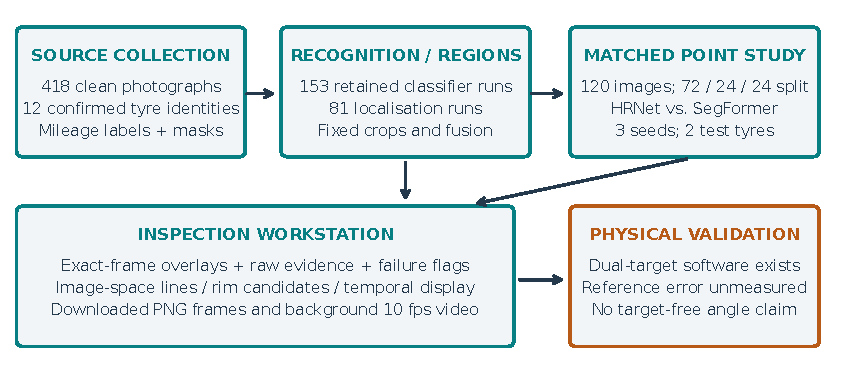
\includegraphics[width=\textwidth]{workflow.pdf}
\caption{Study and workstation overview. The diagram separates completed empirical and software components from physical validation still requiring real reference measurements. The matched geometry study reuses a subset of the source cohort; arrows do not imply independent data collections.}
\label{fig:workflow}
\end{figure*}

\section{Related Work}
\label{sec:related}
\subsection{Physical Measurement and Proxy Recognition}
TireEye uses optical observations of longitudinal groove cross-sections, image edges, and tread-wear indicators as a scale reference \cite{tireeye}. Its relevance here is the distinction between a physically referenced measurement and a classification target. Our mileage labels do not supply the scale or reference measurements needed for an equivalent depth estimate. Consequently, we do not compare our macro-F1 to a millimetre error or claim a physical-wear improvement from a classification score.

Residual networks provide a standard recognition baseline \cite{resnet}, while MobileNetV4 targets efficient architectures across mobile hardware \cite{mobilenet}. We use available implementations and pretrained representations as experimental configurations, not as evidence that one architecture family is universally appropriate for tyres. For models with ordinal heads, CORAL provides a threshold-based formulation for ordered labels \cite{coral}. Its decision rule must be preserved when reconstructing predictions: counting positive ordinal thresholds is not generally interchangeable with taking the largest displayed class score.

\subsection{Explanation and Dense Localisation}
Grad-CAM uses class-related gradients and feature maps to construct coarse localisation maps \cite{gradcam}. Such maps can help identify where a model responds, but visual plausibility alone is insufficient. Parameter-randomisation sanity checks demonstrate why a saliency method must depend meaningfully on learned parameters before it is used as model evidence \cite{sanity}. We combine a project-specific randomisation screen with insertion/deletion diagnostics and explicitly limit the interpretation of spatial saliency ratios.

U-Net, DeepLabV3+, and SegFormer represent different dense-prediction designs \cite{unet,deeplab,segformer}. Our dense-task branch also uses YOLO26 software and a specified RT-DETRv2-R18 model \cite{yolo,rtdetr}. These configurations differ in pretraining, losses, and backend behaviour. A common image set and epoch budget make their outputs comparable within the declared protocol, but do not create a controlled architecture-only experiment. We distinguish the official research papers from mutable software documentation and preserve executed package versions separately.

HRNet maintains high-resolution representations through parallel multiresolution processing \cite{hrnet}. This motivates its use as a boundary-coordinate component, but human-pose benchmarks do not establish tyre performance. Our six fixed-row coordinates, coordinate decoder, and error definition are task-specific. The matched comparator is a newly trained SegFormer on the same geometry split, not a segmentation checkpoint trained on a broader image allocation.

\subsection{Confidence and Geometric Reference Frames}
Temperature scaling addresses confidence calibration without requiring a new recognition backbone \cite{calibration}. Conformal prediction provides a framework for prediction sets under its statistical assumptions \cite{conformal}; coverage observed on a small, dependent collection does not establish deployment coverage. We therefore report achieved coverage, set size, and the limitations of the inherited abstention field.

ChArUco board detection and pose estimation provide the software foundations for the prototype's target-assisted alignment workflow \cite{charuco}. A detected target can define a reference plane only when camera calibration, board scale, orientation, and mounting are appropriate. These assumptions are distinct from segmentation quality. The present contribution integrates the software workflow and exercises synthetic cases; it does not supply the missing real-wheel reference study.

\section{Data and Experimental Design}
\label{sec:data}
\subsection{Collection, Labels, and Sampling Unit}
The preparation audit starts with 888 raw files and removes 470 byte-identical duplicates, leaving 418 clean RGB photographs at $1152\times1536$ pixels. Ten pre-generated derivatives per original produce 4,180 additional files at $768\times768$ pixels. These derivatives are linked to their source images and are not independent observations. The photographs were captured within approximately 22 minutes on August 25, 2026, limiting variation in acquisition conditions.

The low-, mid-, and high-mileage proxy groups contain 169, 97, and 152 clean images, respectively, distributed across 3, 3, and 6 timestamp-derived sessions. Low includes new tyres and the 100--5,000 mileage group; mid includes the 40,000, 70,000, and 90,000 groups; high corresponds to the 100,000-plus group. These are source-group labels, not measured wear severity. The collection operator subsequently confirmed that the 12 sessions represent 12 distinct physical tyres. This statement is recorded as operator confirmation, without an independent identity audit.

\begin{table}[t]
\caption{Historical clean-image allocations. Validation images are reused for internal evaluation; these folds are not an external test set.}
\label{tab:folds}
\centering\small
\begin{tabular}{rrr>{\raggedright\arraybackslash}p{3.15cm}}
\toprule
Fold & Train & Validation & Interpretation\\
\midrule
0 & 232 & 186 & Historical identity-overlap concern\\
1 & 290 & 128 & No listed overlap flag; small internal split\\
2 & 314 & 104 & Historical identity-overlap concern\\
\bottomrule
\end{tabular}
\end{table}

Table~\ref{tab:folds} preserves the existing folds. Folds 0 and 2 carry historical suspected same-tyre overlap flags. The later operator clarification does not constitute an independent re-audit of these allocations, so the flags remain visible. Classification training can use derivatives of training originals; validation uses clean held-out photographs. The dense-task branch uses clean originals only. Results pooled over folds are descriptive internal summaries. Repeating training with three seeds characterises optimisation variation conditional on the same data and does not triple the number of tyres.

\subsection{Manual Regions and Geometry Annotations}
The existing manual label map $M$ defines overlapping binary regions:
\begin{equation}
Y_{\mathrm{tyre}}=\mathbb{1}[M>0],\qquad
Y_{\mathrm{tread}}=\mathbb{1}[M\in\{2,3\}].
\label{eq:masks}
\end{equation}
The tread lies within the tyre; treating these labels as mutually exclusive softmax classes would change the task. Bounding boxes are derived from each region. Model agreement with these masks is not a measurement of inter-annotator consistency: no blind independent repeat-annotation study is available.

The geometry extension contains 120 photographs with 720 visible boundary targets. Each image has a left and right tread coordinate on each of three guide rows at 25\%, 50\%, and 75\% of image height. These targets encode horizontal location at a fixed row, not arbitrary landmarks or three-dimensional orientation. The original 12 pilot photographs are excluded from the 120-image package, but the cohort had already informed development. A frozen allocation uses 72 images from eight tyres for training, 24 from two tyres for validation, and 24 from two tyres for testing. Test identities are \texttt{mileage\_100000\_plus} session 006 and \texttt{new\_tire} session 001. This geometry split is separate from the historical classification folds.

\subsection{Endpoints and Analysis Units}
For classification, we preserve both validation-selected and fixed-final checkpoint statistics. They answer different questions, and selection on the evaluated validation data prevents the larger selected score from being treated as an untouched test result. Localisation and the matched geometry comparison use a fixed epoch-60 endpoint. Unless stated otherwise, numerical differences are descriptive; no population significance claim is inferred from repeated seeds, correlated points, or reused image sets. Missing metrics for a box-only model are undefined rather than zero.

\Needspace{5\baselineskip}
\section{Methods}
\label{sec:methods}
\subsection{Classification, Identity Audit, and Explanation Screening}
The retained classification sweep contains 17 configurations, three folds, and three seeds: 153 runs. Nine additional runs labelled ConvNeXtV2-Small are quarantined because their recorded parameter count and a sampled checkpoint's tensor signature identify a ResNet-18 substitution. These records remain preserved but are excluded from the architecture comparison. Model names alone are therefore insufficient provenance; implementation, initialisation, head, and checkpoint identity are part of the experimental specification.

Macro-F1 averages the class-specific F1 values over the three proxy classes. For an ordinal model with threshold outputs $q_k(x)$, the implemented prediction is
\begin{equation}
\hat y(x)=\sum_{k=0}^{1}\mathbb{1}[q_k(x)>0.5].
\label{eq:ordinal}
\end{equation}
Models trained with a softmax head retain their argmax decision rule. Saved predictions record which rule applies; downstream reconstruction does not replace the ordinal decision with a class-score argmax.

The common classification recipe uses full-frame raw RGB inputs, pretrained full-backbone fine-tuning, a CORAL binary-cross-entropy head, session-balanced sampling, AdamW with initial learning rate $3\times10^{-4}$ and weight decay 0.05, five warm-up epochs, cosine scheduling, and a 60-epoch budget without early stopping. Gradient clipping is 5.0 and training uses half precision. Resolution and batch size follow the architecture registry rather than an identical-resolution assumption: most inputs are 384 pixels, Swin and CoAtNet use 224, and DINOv2 uses 392. Batch sizes range from 16 to 64. Exact per-run configurations and the dataset augmentation policy remain part of the reproducible record.

The explanation screen covers 18 initial candidates and ten shortlist confirmation runs, with 1,208 explanation rows and 35 method-faithfulness rows. A method survives the implemented gate if its randomisation sensitivity exceeds 0.05 and its insertion-minus-deletion area-under-curve value is non-missing. Surviving methods are ranked by that difference. There is no additional requirement that the difference be positive, and passing this gate is not a general certificate of explanation validity.

For a nonnegative saliency map $A$ and tread region $T$, the normalised tread evidence ratio is
\begin{equation}
\mathrm{TER}_{\mathrm{norm}}=
\frac{\sum_{p\in T}A_p/\sum_{p\in\Omega}A_p}{|T|/|\Omega|},
\label{eq:ter}
\end{equation}
where $\Omega$ is the image domain and the ratio is defined only for nonzero denominators. A value above one means concentration beyond the tread's area share. It does not demonstrate causal use of wear features. In this collection, the documented median tread-to-tyre area ratio is 0.990, and 114 images have no visible shoulder. Thus the metric mainly distinguishes tyre from background rather than fine tread from shoulder. Invalid or zero saliency maps remain invalid observations.

The screen selects RegNetY-016, DenseNet-121, and ResNet-50 for one-factor-at-a-time follow-ups. There are 108 discovery runs: three architectures, twelve factor changes, and three seeds on fold 1. A same-fold confirmation stage then evaluates class-weighted sampling, uniform sampling, and random initialisation on ConvNeXtV2-Tiny and MobileNetV4, with three seeds and 60 epochs, giving 18 runs. This tests transfer of factor direction across architectures on the same fold, not independent replication or interactions between separately changed factors.

\subsection{Dense Localisation and Frozen-Classifier Interventions}
The localisation branch comprises nine configurations: U-Net/ResNet-34, DeepLabV3+/ResNet-34, SegFormer-B0, SegFormer-B2, YOLO26-n and YOLO26-s in detection and instance-segmentation modes, and RT-DETRv2-R18. Three folds and three seeds produce 81 runs, each trained for 60 epochs on 512-pixel inputs. The declared optimiser is AdamW with learning rate $10^{-4}$, weight decay 0.01, and cosine scheduling. Batch sizes are four for semantic and YOLO models and two for RT-DETR.

Semantic models use binary cross-entropy plus soft Dice on two sigmoid channels consistent with~\eqref{eq:masks}; the other backends retain their native task losses. Horizontal flipping has probability 0.5 for semantic and repaired YOLO training, while RT-DETR has no online augmentation. YOLO's amended policy disables other hidden augmentations. Final native exponential-moving-average weights are evaluated for YOLO, and final raw weights for the other backends. Differences in pretraining, loss, and backend behaviour are retained as experimental qualifications.

YOLO polygon conversion is verified against the native manual regions. All 836 exported regions meet the required rasterised intersection-over-union (IoU) of at least 0.98; the minimum is approximately 0.980092. This tests the representation conversion, not annotation accuracy. Native masks remain the evaluation reference. Box and mask average precision (AP) use IoU thresholds from 0.50 to 0.95. Region evaluation additionally reports IoU, Dice, and boundary F1 at a two-native-pixel tolerance.

To test downstream usefulness, each localisation run is paired with the frozen final Stage-A ResNet-50 checkpoint of the same fold and seed. Five inputs are evaluated: the full frame, predicted tyre crop, predicted tread crop, oracle tyre crop, and oracle tread crop. Crops include 5\% padding. A missing predicted region causes a recorded full-frame fallback. The classifier is not retrained on crops; therefore changes can reflect both localisation errors and input-distribution shift.

The fusion analysis uses saved probabilities rather than new training. Five fixed arms are evaluated: full frame, tyre only, tread only, equal tyre/tread fusion, and equal full/tyre/tread fusion. For the last arm,
\begin{equation}
\bar{\boldsymbol p}=\tfrac{1}{3}
(\boldsymbol p_{\mathrm{full}}+\boldsymbol p_{\mathrm{tyre}}+
\boldsymbol p_{\mathrm{tread}}).
\label{eq:fusion}
\end{equation}
Class decisions are reconstructed with the saved head semantics. Each arm is paired with the corresponding full-frame result. There are 405 run/arm metric rows and 56,430 image/arm prediction rows. These counts are not numbers of independent tyres or independently trained fusion systems. Fusion weights are fixed rather than selected for a favourable test result.

\subsection{Calibration and Prediction Sets}
The inherited confidence analysis averages the saved probabilities from the three explanation-selected architectures and their three seeds within each fold. Each fold's held-out photographs are stratified into three disjoint image subsets for temperature fitting, conformal calibration, and final diagnostics, using the recorded seed $100+\mathrm{fold}$. This subdivision is image-level, not a new tyre-disjoint split. Temperature is fitted by minimising negative log-likelihood on the first subset. Expected calibration error uses 15 equal-width confidence bins. Unlike the standalone ordinal decision in~\eqref{eq:ordinal}, this inherited ensemble diagnostic explicitly uses the argmax of its averaged class probabilities.

Conformal nonconformity is $1-p_y$ on the separate calibration subset. The implementation uses the higher empirical quantile at $\min\{1,\lceil(n_{cal}+1)0.9\rceil/n_{cal}\}$ and includes test class $k$ when $1-p_k$ does not exceed that threshold. Coverage and mean set size are then measured on the third subset. The recorded abstention rate counts sets larger than one, leaving empty sets outside that field. We preserve this implementation detail rather than interpreting the field as a complete reject-option metric.

\subsection{Matched Boundary Learning}
The HRNet adapter projects its four feature maps to 16 channels each, upsamples them to the highest feature resolution, concatenates them, and produces six coordinate-logit maps. Bilinear sampling at the fixed guide rows yields a horizontal distribution for each point. The target Gaussian has standard deviation 1.5 feature pixels; training minimises mean cross-entropy with the normalised target distribution. Decoding takes the softmax-weighted expected horizontal coordinate, scaled back to native width minus one. Vertical position is prescribed by the guide, not estimated by the network.
HRNet-W18 predicts six horizontal coordinates using Gaussian coordinate targets. The matched SegFormer-B0 learns the two overlapping manual mask channels from the same 72 training images; validation/test dense masks do not enter its training loader. Both use input height/width $512/384$, batch size two, AdamW with learning rate $10^{-4}$ and weight decay 0.01, cosine epoch scheduling, no augmentation, frozen batch-normalisation running statistics, three seeds, and epoch 60 for final comparison. Parameter counts are 9,603,962 and 3,714,658, respectively. The supervision and pretrained backbones differ, so a matched split and budget do not isolate architecture as a causal factor.

SegFormer logits are bilinearly interpolated to native resolution and thresholded at sigmoid 0.5. Tread-row extrema supply left/right points; empty rows and frame-clipped extrema are rejected. The declared full-set evaluation replaces a missing point with a training-only mean coordinate and separately reports raw coverage and conditional error. This prevents silent evaluation on an easier detected subset. No replacement is needed in the final comparison.

For image $i$ with native width $W_i$, target $j$, and training seed $s$, the horizontal error is
\begin{equation}
e_{ijs}=\frac{|\hat x_{ijs}-x_{ij}|}{W_i-1},\qquad
E_s=\frac{1}{6N}\sum_{i=1}^{N}\sum_{j=1}^{6}e_{ijs},
\label{eq:error}
\end{equation}
where $N=24$ test images. The reported percentage is $100E_s$. Each seed contributes 144 target points, giving 432 paired records across seeds on the same two tyres. Relative error reduction uses the SegFormer mean as denominator, not the number of correctly classified images. The mean over seeds is not an evaluated ensemble.

\subsection{Inspectable Geometry and Target-Assisted Alignment}
\label{sec:geometry}
The workstation applies the deployed models to the exact displayed analysis frame. Orientation follows the video metadata and the established portrait policy. HRNet and matched SegFormer use seed 1, final epoch 60, with full-image resizing, ImageNet normalisation, and no test-selected crop or rotation search. Local inference uses full precision; the saved training evaluation used automatic mixed precision. Adapter checks therefore verify coordinate/preprocessing consistency without claiming a new aggregate benchmark reproduction.

Image geometry is fitted to observed image evidence rather than obtained by translating class scores into angles. A segmentation mask guides the search region. The boundary path samples Canny edges near the two silhouette sides and uses deterministic consensus followed by least-squares fits of $x=ay+b$. Accepted supports must be sufficiently long and consistent; disagreeing sides, collapsed fits, fragmented masks, and clipping can withhold the fit. A separate side-view mode fits an inner ellipse candidate only when image-edge support and angular coverage are sufficient. A tyre silhouette is not automatically called a rim. Accepted side lines yield an image-space midpoint line, not camber or toe.

Temporal display tracking smooths consistent proposals and resets on discontinuities, source changes, or invalid results. Raw learned coordinates remain available, and crossed or missing boundaries receive review flags. A stable display is not treated as evidence of accuracy. The explanation view distinguishes the predicted search outline from accepted edges and explicitly labels a withheld fit.

The physical-measurement path instead requires calibrated camera intrinsics and two separately identified ChArUco targets \cite{charuco}. The ground target defines the reference frame and the wheel target supplies a candidate wheel-plane normal. With vehicle axes $X$ forward, $Y$ left, and $Z$ up, and outward-facing normal $\boldsymbol n$ after the wheel-side convention is applied, the implemented angles are
\begin{align}
\gamma &= \operatorname{atan2}(-n_z,\sqrt{n_x^2+n_y^2}),\\
\tau &= \operatorname{atan2}(n_x,|n_y|),
\label{eq:angles}
\end{align}
for camber and toe-in under that explicit setup convention. The workflow requires setup confirmation and rejects missing or unsuitable pose evidence. These equations are software definitions contingent on target orientation and wheel-plane mounting; they do not validate physical accuracy. Real fixture alignment, reference measurements, and remount/runout studies remain necessary.

\subsection{Execution and Reproducibility}
\begin{figure}[t]
\centering
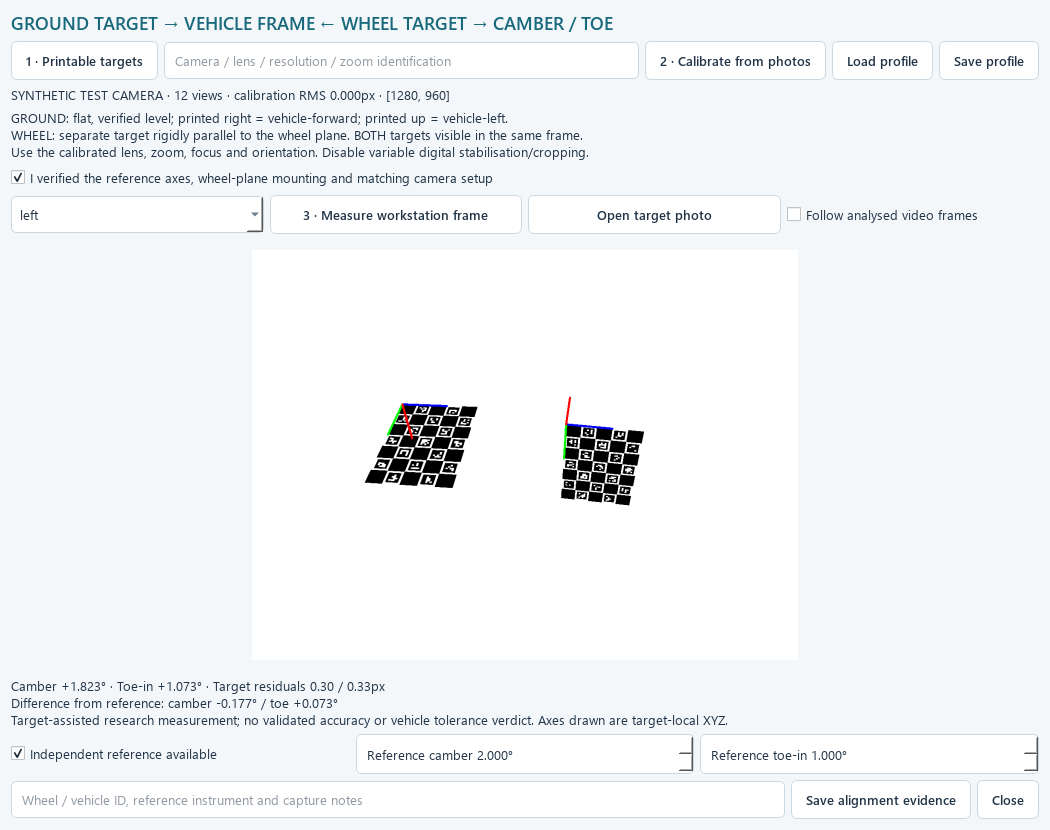
\includegraphics[width=\columnwidth]{alignment-bench-check.png}
\caption{Target-assisted alignment interface exercised with a \emph{synthetic test camera}. The displayed angles and residuals are software-test outputs from rendered targets, not measured accuracy on a physical wheel.}
\label{fig:alignment}
\end{figure}

Kaggle sessions provide training compute and Hugging Face stores persistent records. Jobs retain model/optimiser state, scheduler and scaler state where applicable, random-number-generator state, and execution position. The older dense engine resumes completed epochs; the later geometry engine checkpoints completed optimiser steps and the next-batch cursor. Normal publication is batched at roughly 30-minute intervals, with major completion and catchable interruption requesting a flush. Remote rate limits, failed uploads, or a forced operating-system kill can still lose unpublished progress.

The geometry engine's deterministic resizing repair passed a Tesla T4 resume check with zero maximum parameter difference. This verifies that exercised interruption path, not every possible hardware failure. Immutable revisions and hashes identify the reviewed artifacts. The present paper regenerates its numeric tables and plots from those frozen local records; it does not rerun training or claim independent replication of the original experiments.

\section{Results}
\label{sec:results}
\subsection{Classification Is Sensitive to Fold and Endpoint}
Simple baselines reveal substantial fold dependence. The colour probe obtains macro-F1 values of 0.88696, 0.46405, and 0.12322 on folds 0, 1, and 2. The histogram-of-oriented-gradients support-vector machine obtains 0.79602, 0.18182, and 0.98412. These patterns motivate scrutiny of capture-specific cues, but do not identify a unique shortcut mechanism. A historical random-initialised ResNet-18 trained for 15 epochs averages 0.82135, whereas the later matched nine-run, 60-epoch ResNet-50 control averages 0.82332 at the final endpoint. The two controls differ in backbone and budget and are not interchangeable.

Table~\ref{tab:architectures} and Fig.~\ref{fig:endpoints} show the retained sweep. MobileNetV4 has a selected mean macro-F1 of 0.99746 and final mean of 0.91310. The endpoint gap is larger for EfficientNetV2-S (0.97615 versus 0.70874) and VGG16-BN (0.89194 versus 0.45870), while ConvNeXtV2-Tiny is comparatively stable (0.90891 versus 0.90238). Consequently, a near-perfect selected score cannot stand alone as a performance summary. These values include the historically flagged folds and do not establish external generalisation, physical-wear recognition, or the optimal checkpoint policy for new tyres.

\begin{table}[t]
\caption{Archival classification summary in alphabetical order. Each row averages nine runs (three grouped folds and three seeds). These internal validation summaries are retained for completeness; fold-specific analysis is primary.}
\label{tab:architectures}
\centering
\small
\setlength{\tabcolsep}{4pt}
\begin{tabular}{lrr}
\toprule
Architecture & Selected & Final \\
\midrule
CLIP ViT-B/16 & 0.95076 & 0.78897 \\
CoAtNet-0 & 0.80537 & 0.72041 \\
ConvNeXtV2-T & 0.90891 & 0.90238 \\
DeiT-III-S & 0.74726 & 0.72855 \\
DenseNet-121 & 0.89660 & 0.83852 \\
DINOv2-B & 0.91277 & 0.88380 \\
DINOv2-S & 0.87346 & 0.78842 \\
EfficientNetV2-S & 0.97615 & 0.70874 \\
MaxViT-T & 0.92189 & 0.85982 \\
MobileNetV4 & 0.99746 & 0.91310 \\
RegNetY-016 & 0.93495 & 0.74087 \\
ResNet-50 & 0.93651 & 0.82922 \\
ResNeXt-50 & 0.92260 & 0.76566 \\
Swin-S & 0.95259 & 0.85744 \\
Swin-T & 0.97673 & 0.83478 \\
VGG16-BN & 0.89194 & 0.45870 \\
ViT-S & 0.93235 & 0.75858 \\
\bottomrule
\end{tabular}
\end{table}

\begin{figure*}[t]
\centering
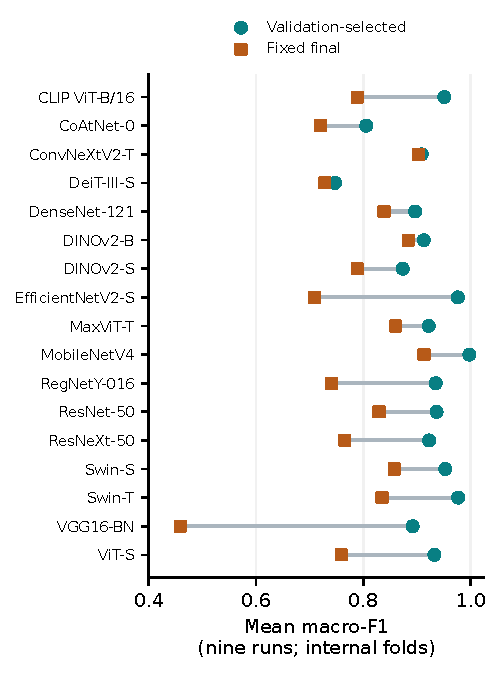
\includegraphics[width=.88\textwidth]{endpoints.pdf}
\caption{Validation-selected and fixed-final macro-F1 means for all 17 retained configurations. Each point averages nine runs on the same historical folds; connecting segments highlight endpoint differences and are not uncertainty intervals. No test-set architecture ranking is implied.}
\label{fig:endpoints}
\end{figure*}

\subsection{Explanation Diagnostics and Same-Fold Confirmation}
The inherited hypothesis that normalised tread evidence predicts cross-fold stability better than accuracy is not supported: the recorded primary and reference statistics are 0.42710 and 0.90743, respectively, across ten entries. This analysis uses legacy selected-endpoint statistics and is not relabelled as a fixed-budget result. The marking/damage hypothesis is inconclusive or undefined, and the fine-grained architecture hypothesis remains untested because its planned model arms are absent. In particular, fold-1 marking removal operates on zero active marking images; its near-zero effect cannot establish marking independence.

Table~\ref{tab:confirmation} reports the confirmation stage. Random initialisation is negative for both architectures at both endpoints. Class-weighted sampling has a positive selected effect for ConvNeXtV2-Tiny but a negative selected effect for MobileNetV4, while both final effects are positive. Uniform sampling is not consistently beneficial. The supported interpretation therefore specifies architecture, endpoint, and the existing fold. The experiment neither isolates factor interactions nor establishes a population-level sampling benefit.
\begin{table}[t]
\caption{Same-fold confirmation: mean macro-F1 change relative to each matched baseline over three seeds. Selection and final endpoints can give different sampling conclusions.}
\label{tab:confirmation}
\centering
\small
\setlength{\tabcolsep}{4pt}
\begin{tabular}{llrr}
\toprule
Architecture & Factor & $\Delta$ selected & $\Delta$ final \\
\midrule
ConvNeXtV2-T & Class-weighted & +0.01257 & +0.02396 \\
ConvNeXtV2-T & Uniform & +0.00000 & +0.01027 \\
ConvNeXtV2-T & Random init. & -0.42857 & -0.38737 \\
MobileNetV4 & Class-weighted & -0.02839 & +0.01886 \\
MobileNetV4 & Uniform & -0.06959 & -0.17079 \\
MobileNetV4 & Random init. & -0.37150 & -0.27525 \\
\bottomrule
\end{tabular}
\end{table}


\subsection{Region Overlap and Boundary Fidelity Differ}
All 81 localisation runs complete 60 epochs and evaluation, corresponding to 4,860 epoch records. Table~\ref{tab:localisation} restricts the principal summary to fold 1; this avoids treating flagged-fold averages as the main estimate but does not make fold 1 an external test. Semantic models have tread IoU between approximately 0.972 and 0.976, whereas their two-pixel boundary F1 is approximately 0.358--0.374. YOLO instance-segmentation models obtain tread IoU near 0.856--0.858 and boundary F1 near 0.189--0.226.

Figure~\ref{fig:localisation} makes the metric distinction explicit. Region overlap rewards agreement across a large interior area; boundary F1 is sensitive to contour displacement under its narrow tolerance. Neither metric alone establishes that the model has recovered the information needed for proxy classification, let alone physical tread condition. The evaluation is against one existing manual reference set rather than an independently repeated annotation standard.
\begin{table*}[t]
\caption{Fold-1 localisation means over three seeds. AP denotes COCO-style AP at IoU thresholds 0.50:0.95. Boundary F1 uses a two-native-pixel tolerance. Dashes denote undefined mask metrics for box-only models.}
\label{tab:localisation}
\centering
\small
\setlength{\tabcolsep}{4pt}
\begin{tabular}{lrrrr}
\toprule
Model & Box AP & Mask AP & Tread IoU & Boundary F1 \\
\midrule
DeepLabV3+/R34 & 0.98612 & 0.99675 & 0.97176 & 0.35988 \\
RT-DETRv2-R18 & 0.94073 & -- & -- & -- \\
SegFormer-B0 & 0.91189 & 0.99836 & 0.97372 & 0.37258 \\
SegFormer-B2 & 0.97657 & 0.99982 & 0.97569 & 0.37412 \\
U-Net/R34 & 0.91413 & 0.99704 & 0.97216 & 0.35820 \\
YOLO26-n det. & 0.95278 & -- & -- & -- \\
YOLO26-n seg. & 0.95204 & 0.95890 & 0.85815 & 0.18926 \\
YOLO26-s det. & 0.96081 & -- & -- & -- \\
YOLO26-s seg. & 0.95227 & 0.96215 & 0.85627 & 0.22623 \\
\bottomrule
\end{tabular}
\end{table*}

\begin{figure*}[t]
\centering
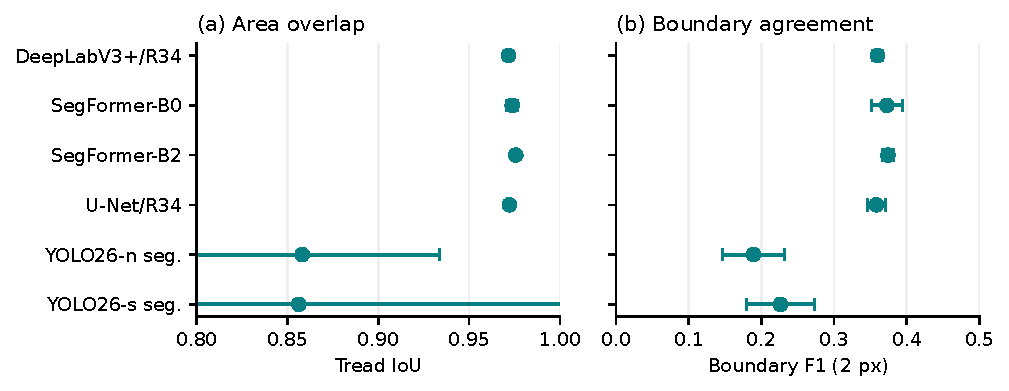
\includegraphics[width=\textwidth]{localisation.pdf}
\caption{Fold-1 semantic/instance-segmentation results: (a) tread IoU and (b) boundary F1 at two native pixels. Points are means and whiskers are sample standard deviations across three training seeds. The panels deliberately use different horizontal scales. Seed variation is not a confidence interval over independent tyres.}
\label{fig:localisation}
\end{figure*}

\subsection{Predicted Crops and Fixed Fusion Have Negative Mean Effects}
The paired frozen-classifier analysis does not show an overall gain from the predicted crops. Mean macro-F1 changes are -0.01257 for tyre-only and -0.01467 for tread-only inputs across the 81 localisation source runs. These means do not imply that every configuration/fold pair worsens. They quantify the declared intervention on a classifier trained for full-image inputs, with no crop-specific retraining.

Fixed probability fusion also has negative mean effects (Table~\ref{tab:fusion}, Fig.~\ref{fig:fusion}). Equal tyre/tread fusion gives -0.01568; equal full/tyre/tread fusion gives -0.01324. The latter is a decrease of about 1.324 macro-F1 percentage points, not a 1.324\% relative error reduction. The result argues against assuming that localisation or additional views automatically help an existing classifier. Lost context, changed scale, crop distribution shift, localisation errors, and correlated predictions are plausible explanations, but the present design does not separate their contributions. Crop-trained recognition and learned fusion would require new experiments.
\begin{table}[t]
\caption{Fixed probability fusion: mean paired macro-F1 changes over 81 source runs. Repeated images and shared classifiers make these rows dependent.}
\label{tab:fusion}
\centering
\small
\setlength{\tabcolsep}{4pt}
\begin{tabular}{lrr}
\toprule
Arm & Rows & Mean $\Delta$ \\
\midrule
Full frame & 81 & +0.00000 \\
Tyre only & 81 & -0.01257 \\
Tread only & 81 & -0.01467 \\
Tyre + tread & 81 & -0.01568 \\
Full + tyre + tread & 81 & -0.01324 \\
\bottomrule
\end{tabular}
\end{table}

\begin{figure}[t]
\centering
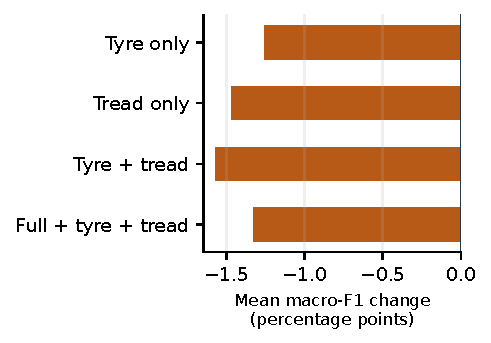
\includegraphics[width=\columnwidth]{fusion.pdf}
\caption{Mean paired changes from the full-frame classifier for four fixed crop/fusion arms. Bars average 81 dependent source runs; no independent-sample uncertainty or favourable-arm selection is implied.}
\label{fig:fusion}
\end{figure}

\subsection{Confidence Diagnostics Are Fold-Dependent}
Temperature scaling leaves the recorded macro-F1 unchanged and reduces confidence-error metrics on the retained calibration-test subsets (Table~\ref{tab:calibration}). On fold 1, expected calibration error decreases from 0.18955 to 0.07377, and negative log-likelihood from 0.35630 to 0.16226, with 41 test images. Extremely small calibrated errors on the flagged folds are not evidence of deployment-grade certainty.

At nominal 90\% coverage, the observed conformal coverages are 0.86885, 0.97561, and 0.93939 on folds 0, 1, and 2, respectively (Table~\ref{tab:conformal}). Thus only fold 0 is below nominal in these observed subsets. Mean set sizes below one on folds 0 and 2 imply empty sets. The inherited abstention field does not count all empty-set events and cannot be presented as a complete rejection policy. Small subset sizes, dependent acquisition, and reuse of internal evidence constrain generalisation of these diagnostics.
\begin{table}[t]
\caption{Confidence diagnostics on held-out calibration-test subsets. ECE is the recorded expected calibration error; values near zero on internal folds do not imply external reliability.}
\label{tab:calibration}
\centering
\small
\setlength{\tabcolsep}{4pt}
\begin{tabular}{llrrrr}
\toprule
Fold & Scores & $n$ & F1 & ECE & NLL \\
\midrule
0 & Raw & 61 & 1.0000 & 0.2115 & 0.2425 \\
0 & Temp. & 61 & 1.0000 & 0.0000 & 0.0000 \\
1 & Raw & 41 & 0.8030 & 0.1896 & 0.3563 \\
1 & Temp. & 41 & 0.8030 & 0.0738 & 0.1623 \\
2 & Raw & 33 & 1.0000 & 0.1293 & 0.1438 \\
2 & Temp. & 33 & 1.0000 & 0.0000 & 0.0000 \\
\bottomrule
\end{tabular}
\end{table}

\begin{table}[t]
\caption{Prediction-set diagnostics at nominal 90\% coverage. The recorded abstention field does not count every empty-set event.}
\label{tab:conformal}
\centering
\small
\setlength{\tabcolsep}{4pt}
\begin{tabular}{rrrrrr}
\toprule
Fold & $n_{cal}$ & $n_{test}$ & Coverage & Set size & Abstain \\
\midrule
0 & 62 & 61 & 0.8689 & 0.8689 & 0.0000 \\
1 & 43 & 41 & 0.9756 & 1.0976 & 0.0976 \\
2 & 35 & 33 & 0.9394 & 0.9394 & 0.0000 \\
\bottomrule
\end{tabular}
\end{table}


\subsection{Matched Point Learning Reduces Still-Image Error}
Table~\ref{tab:geometry} reports the fixed-final comparison, independently recomputed here from the 432 paired point records. Mean horizontal error is 1.312\% of native width for HRNet and 1.721\% for matched SegFormer, corresponding to approximately 15.10 and 19.80 native pixels. The absolute difference is 0.409 percentage points of width, or 4.70 pixels. Relative to the SegFormer mean, HRNet reduces error by 23.75\%. SegFormer raw coverage is 100\%, with zero fallback substitutions, so its raw and fallback-assisted means coincide.

HRNet has lower mean error in every seed and on each of the two test tyres (Fig.~\ref{fig:geometry}). This does not mean every individual point improves. The new-tyre example has higher error for both models than the high-mileage example, but two tyres cannot establish a class effect. The result supports HRNet as a candidate point-localisation component within this matched study. It does not establish an architecture-only advantage because supervision and initial representations differ, nor does it demonstrate downstream classification improvement or physical-angle accuracy.
\begin{table}[t]
\caption{Matched fixed-epoch-60 horizontal point error (\% of native width minus one). Each seed uses the same 24 images from two test tyres; coverage is the SegFormer raw point coverage.}
\label{tab:geometry}
\centering
\small
\setlength{\tabcolsep}{4pt}
\begin{tabular}{lrrr}
\toprule
Seed & HRNet & SegFormer & Coverage (\%) \\
\midrule
1 & 1.391 & 1.788 & 100 \\
2 & 1.284 & 1.705 & 100 \\
3 & 1.261 & 1.668 & 100 \\
Mean & 1.312 & 1.721 & 100 \\
\bottomrule
\end{tabular}
\end{table}

\begin{figure*}[t]
\centering
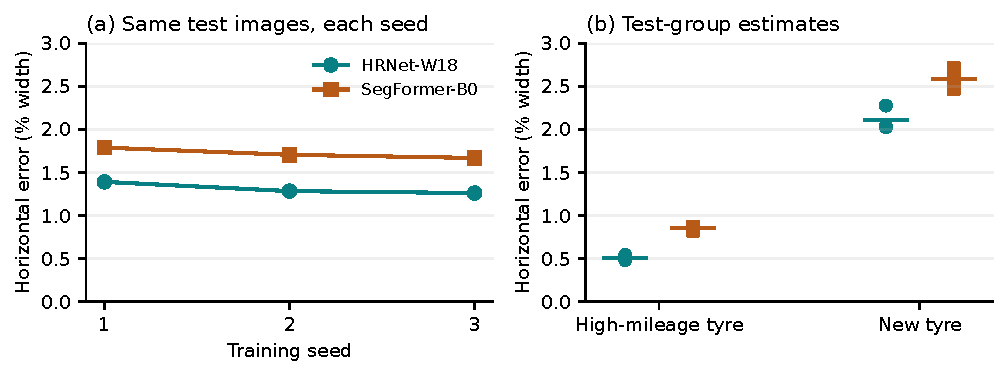
\includegraphics[width=\textwidth]{geometry.pdf}
\caption{Matched boundary comparison. (a) Mean horizontal error for each training seed on the same 24 images. (b) Per-tyre error, retaining all three seed values; horizontal marks are seed means. HRNet is lower in each seed/tyre comparison. These observations are correlated and provide no independent-tyre significance interval.}
\label{fig:geometry}
\end{figure*}

\subsection{Workstation Integration and Observed Video Failures}
Tread Station is a native PySide6/PyTorch application with photo/video loading, portrait-aware playback, asynchronous inference, comparison, geometric overlays, and saved evidence restoration. Existing classifier and region checkpoints remain separate from the optional HRNet/matched-SegFormer geometry components. An inference result is attached to its analysed frame; a newer live preview is shown separately rather than receiving a stale mask. Figure~\ref{fig:station} shows the implemented interface, and Fig.~\ref{fig:qualitative} pairs an operational still example with a preserved video failure.

The saved adapter checks cover strict checkpoint loading, preprocessing, coordinate decoding, repeatability, blank-input flags, temporal resets, and immutable source pixels. A local check on one internal still measured five warm inference calls on an NVIDIA GTX 1650. HRNet's median was 72.60 ms (range 51.41--88.46 ms); matched SegFormer's median was 33.48 ms (33.32--33.84 ms). These timings include preprocessing, inference, extraction, and GPU synchronisation, but exclude model loading and file decoding. Peak allocated memory in the two-component check was approximately 182 MiB. These small operational samples are not a controlled training-hardware comparison, sustained camera throughput, or a guaranteed frame rate.

The supplied videos expose crossed or collapsed HRNet boundaries, missing matched boundaries, and disagreement between models. Crossed pairs withhold widths and connecting geometry while retaining raw proposals for review. No video point ground truth is available, so the passing playback/UI tests establish software behaviour rather than localisation accuracy. Temporal smoothing cannot correct a systematically wrong proposal, and still-image gains cannot be transferred to video by assertion.

The workstation additionally exports the shown analysed frame as PNG and processes an opened video separately at ten output frames per second. The latter runs with a separate CPU engine and frozen display/recipe settings, leaving the GPU available for inspection. The software checks cover frame selection, output duration, portrait dimensions, cancellation, and incomplete-output cleanup; a short real-model portrait excerpt verifies the complete export path. Export frame rate describes the saved playback, not inference speed. This facility supports evidence sharing and does not add an accuracy result.

\begin{figure*}[t]
\centering
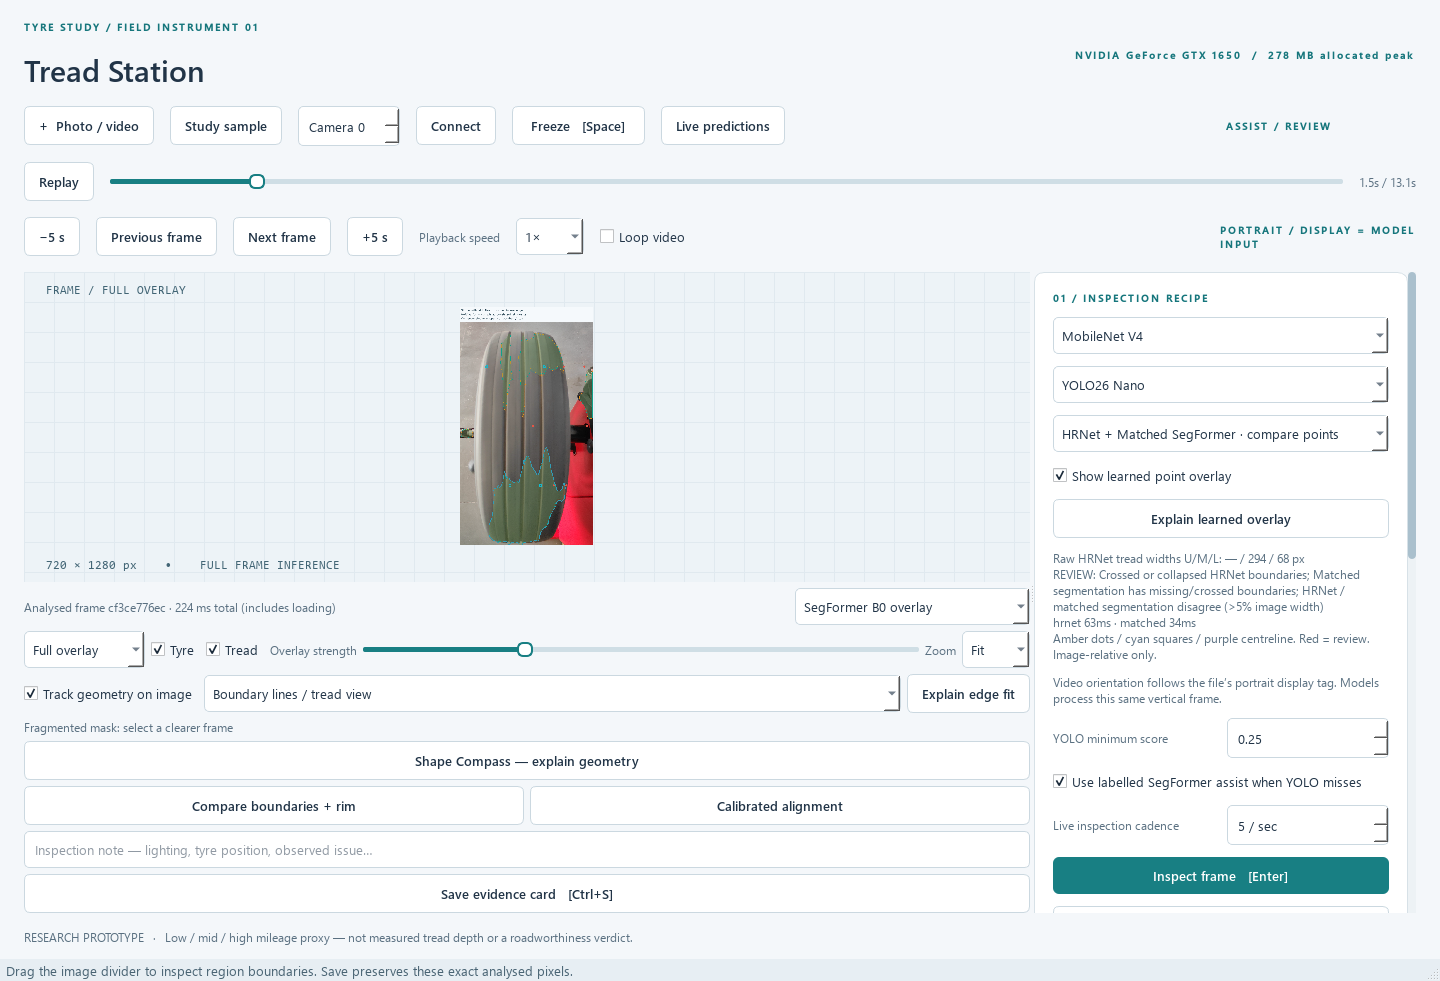
\includegraphics[width=.92\textwidth]{video1-learned-workstation.png}
\caption{Saved native workstation view with learned geometry enabled. This operational screenshot predates the additional download controls. The inspected frame, source preview, model observations, and review flags are distinct. Interface completion is not field-accuracy validation.}
\label{fig:station}
\end{figure*}

\begin{figure*}[t]
\centering
\begin{minipage}[t]{.45\textwidth}
\centering
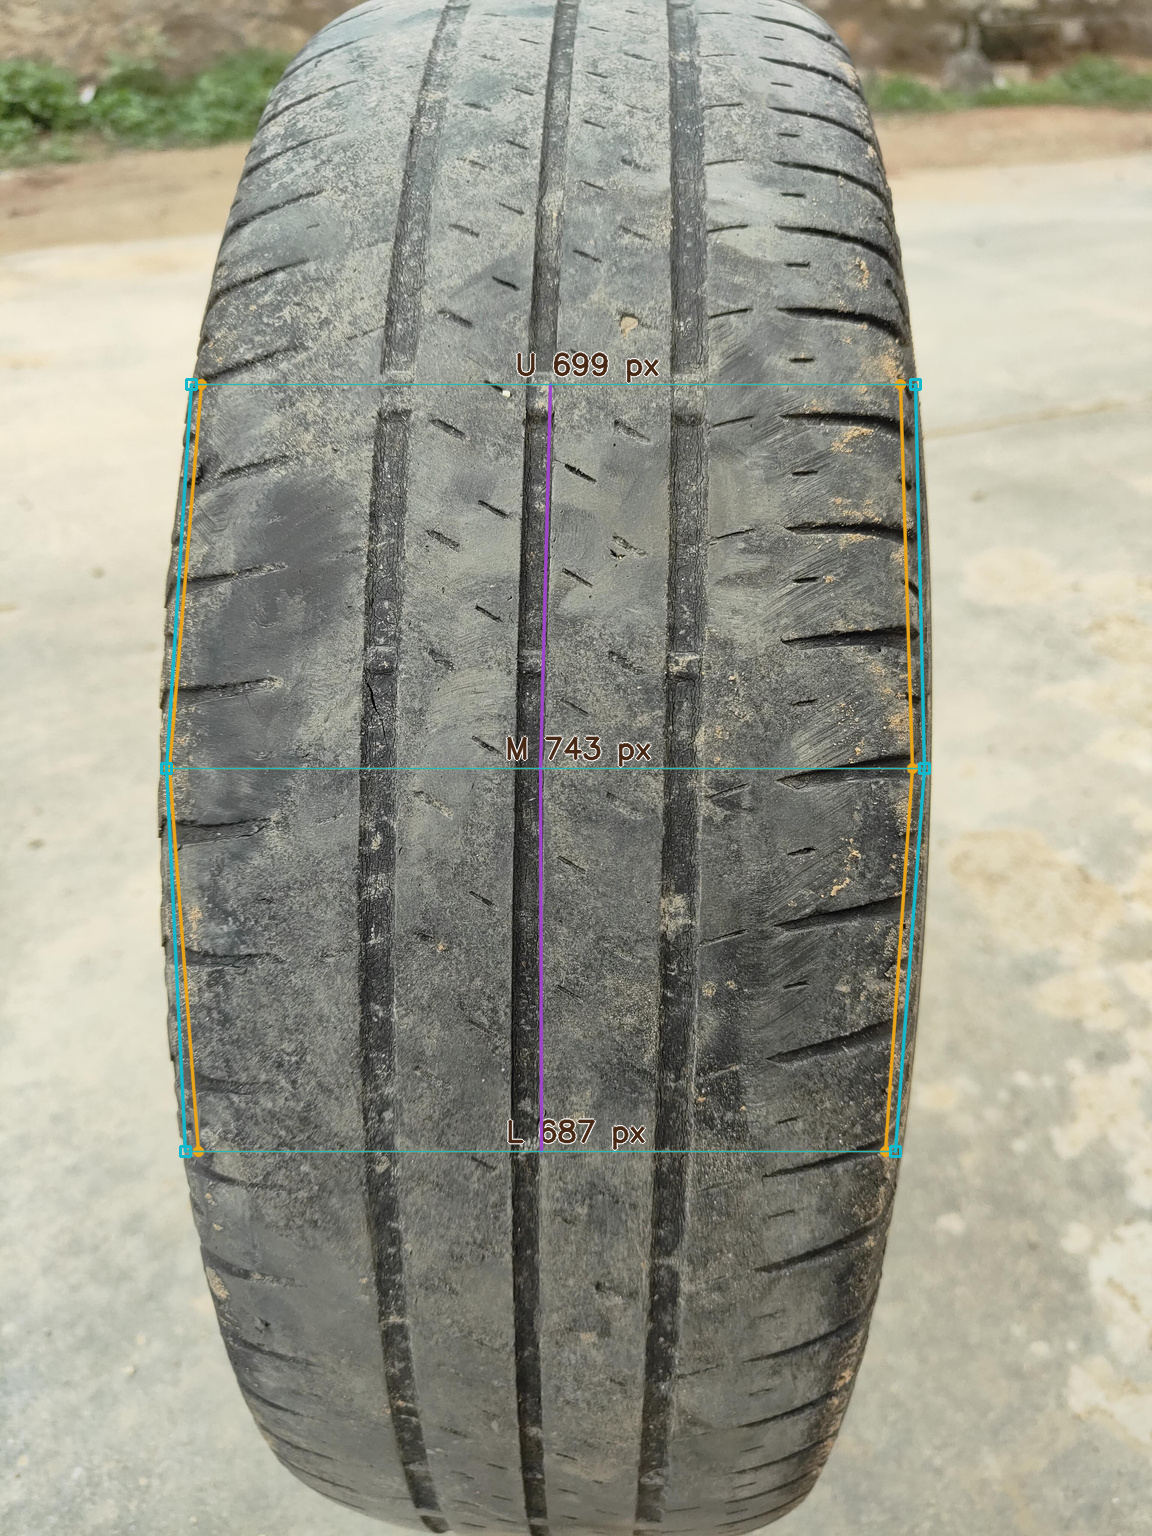
\includegraphics[width=\linewidth,height=6cm,keepaspectratio]{learned-image-check.png}\\
\small (a) Selected internal still-image check
\end{minipage}\hfill
\begin{minipage}[t]{.52\textwidth}
\centering
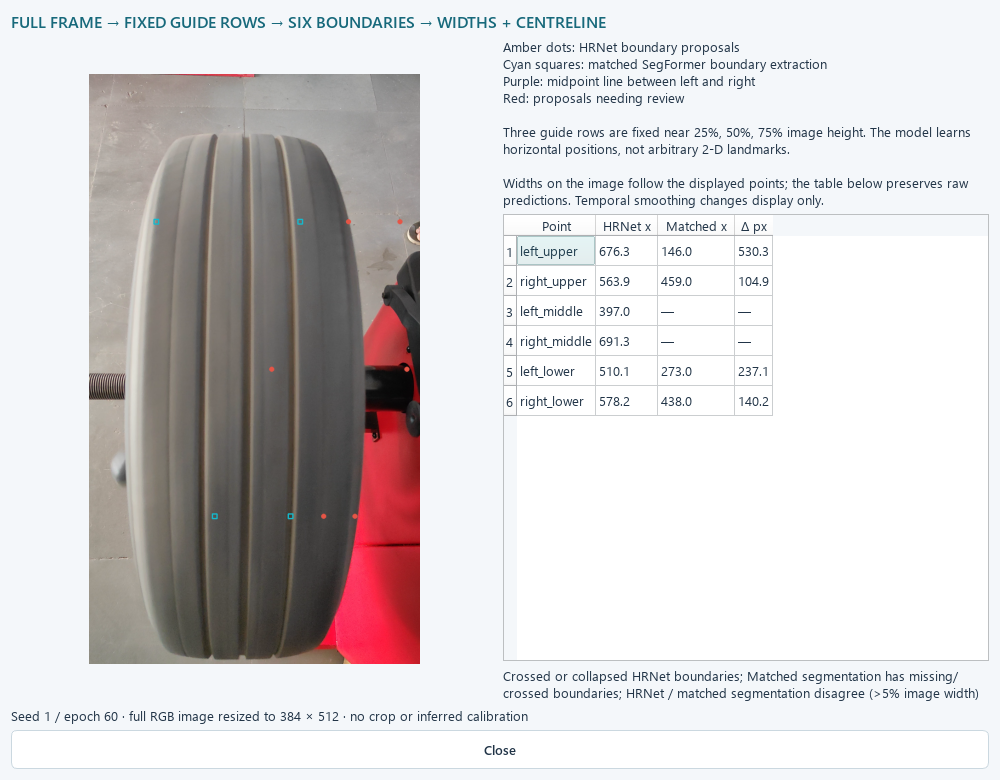
\includegraphics[width=\linewidth,height=6cm,keepaspectratio]{video1-learned-diagram.png}\\
\small (b) Preserved video-domain failure
\end{minipage}
\caption{Qualitative operational evidence, not a new held-out benchmark. Amber HRNet proposals, cyan matched-SegFormer points, and the image-space centreline are shown on the still. The video explanation retains crossed/missing boundaries and disagreement rather than concealing failure. All widths and slopes are image-relative. The images are reproduced from the saved integration checks without altering predicted coordinates.}
\label{fig:qualitative}
\end{figure*}

\subsection{Alignment Software Is Tested Synthetically}
The target-assisted interface generates distinct ground/wheel boards, creates or loads a camera profile, solves target poses, applies the declared side convention, and records signed outputs with pose residuals. It also accepts an independent reference reading for comparison. Synthetic tests exercise known poses, both wheel sides, missing targets, scaling/orientation, setup gating, and evidence export (Fig.~\ref{fig:alignment}). The supplied videos do not contain this calibrated dual-target setup. No result here measures real wheel-angle error, fixture mounting error, or runout compensation.

\section{Discussion}
\label{sec:discussion}
\subsection{Answers to the Research Questions}
\textit{RQ1: checkpoint policy and held-out group.} The fold-specific analysis shows that a pooled near-perfect selected score can obscure a materially weaker fixed-final result on one group allocation. Reporting F1 with class-index MAE and QWK makes the type of error more interpretable. The group audit also resolves a reporting ambiguity: recorded session membership is disjoint, whereas the historical identity warning concerns visual resemblance between two operator-confirmed different tyres. These are different issues and should not be conflated. Checkpoint selection still uses the evaluated validation fold.

\textit{RQ2: localisation as an intervention.} Region agreement does not ensure a downstream gain for a classifier trained on full frames. The fold-specific intervention table localises the overall negative mean: fold 1 worsens, fold 0 is unchanged, and fold 2 has small improvements. This is stronger evidence than either assuming crops help or claiming crops universally harm. It identifies a limitation of this frozen-classifier intervention. A crop-trained classifier or learned fusion could behave differently and requires its own controlled evaluation. Boundary F1 and IoU describe complementary spatial properties, consistent with prior boundary-sensitive evaluation work.

\textit{RQ3: boundary representation.} Point learning improves the average matched error, while the image-level and location-level analyses show nonuniform benefit. The left-middle location changes little and two image averages favour mask-derived boundaries. Both models remain potentially useful: dense masks provide a search region, while point predictions provide direct coordinate proposals. The study compares complete supervised pipelines; it does not identify the backbone, loss, or pretraining source as the cause of the difference.

These results support an evaluation practice: preserve the reference prediction, pair each intervention with it, report the actual decision rule and coverage, and retain invalid cases. The new gate analysis further shows that explanation-guided model eligibility is sensitive to a stricter heuristic threshold. This strengthens the methodological account without turning an exploratory shortlist into a robust selection guarantee.

\subsection{Scope of the Evidence}
The data section states the independent grouping and acquisition scope once, and all results retain that interpretation. Repeated images, seeds, and point coordinates remain correlated. The classification folds cover the available groups but are internal, and the fixed geometry test covers two of those groups. Re-analysis can reveal conditional effects and errors; it cannot create additional subjects or a prospectively untouched test set. No p-value or population confidence interval is therefore computed from the 432 point records as if they were independent tyres.

Mileage categories are proxies, not measured tread depth or roadworthiness. Tread design, background, illumination, or capture conditions may contribute to prediction; the baseline variation motivates that concern but does not identify its cause. The available manual labels lack a blinded repeat-annotation estimate. The point-versus-mask comparison differs in supervision, pretrained representations, and capacity. These limits define the applicable conclusions rather than invalidate the observed paired results.

Video examples expose failure but have no labelled prevalence estimate. Local timing checks do not establish sustained throughput. Target-assisted alignment is software with synthetic tests; a real reference-angle experiment is required for physical accuracy. The article consequently centres on image-space evaluation and does not use alignment screenshots as measurement results.

\subsection{Experiments That Would Add Independent Evidence}
The highest-value next boundary experiment is rotating held-out tyre groups with frozen model settings and fresh training for each split, while retaining a separate development allocation. Existing checkpoints cannot be evaluated on their training tyres and relabelled as cross-validation. A shared-backbone point-versus-mask ablation would separate representation from backbone more directly. Both require additional training; they are not small post-processing analyses and were not executed for this revision.

A blinded second annotation pass on a stratified subset would estimate label repeatability. A tyre-disjoint labelled video set would permit missing-boundary, crossing, point-error, and temporal-consistency rates. Physical claims require depth or wheel-angle references with repeated mounting and runout assessment. These studies address different uncertainties; adding more architectures on the same split would not substitute for them.

\section{Artifact Availability and Reproducibility}
\label{sec:artifacts}
Source code and documentation are available at
\url{https://github.com/Shanmuk4622/tyre-wear-alignment-cv}.
Persistent study artifacts are at
\url{https://huggingface.co/datasets/Shanmuk4622/tyre-wear-study}.
The reporting snapshot is pinned to
\path{22d5a6bc9f953ba3bf2a75919edc7db3193b317b}; the HRNet report to
\path{a92c0f9c5c1b78c6a06e13d51e18722195230658}; and the matched comparison to
\path{bbe586c6f00cf12ae4cac8b2e9cb4f875b272abb}.

The manuscript package includes numerical source hashes and a repeatable revision analysis. The latter checks split membership, reconstructs endpoints from 18 complete epoch histories, repeats explanation-gate decisions, and aggregates paired boundary and fusion records. These are analyses of frozen results, not new training runs. The revision report records every reviewer issue, the implemented response, and remaining evidence needs.

Relevant dense-task versions include Ultralytics 8.4.20, Transformers 4.51.3, segmentation-models-pytorch 0.5.0, and timm 1.0.15. Local integration uses PyTorch 2.5.1 with CUDA 12.1 and OpenCV 4.11.0. Per-phase environments, data lineage, frozen notebooks, and model identities remain necessary for scientific reproduction; a successful paper build alone is not a replication of training.

\section{Conclusion}
The study evaluates three links in a vision-based tyre inspection workflow: checkpoint policy, localisation interventions, and boundary representation. Fold-specific ordinal diagnostics show that pooled selected scores obscure checkpoint and group dependence. Predicted crops and fixed fusion reduce the frozen classifier's mean F1 overall, with the effect concentrated on one fold. Point learning reduces matched horizontal error by 23.75\% relative to mask-derived boundaries and improves 22 of 24 image averages, with complete comparator point coverage. The gain describes the stated pipelines and fixed evaluation cohort. These results support traceable component evaluation and failure visibility; broader transfer and physical measurement remain separate validation tasks.

\section*{Acknowledgment}
No external funding was received for this work. OpenAI Codex~\cite{codex} was used extensively to assist initial drafting and revision of the abstract, Sections I--VIII, appendices, captions, and analysis/build code, including literature organisation, language editing, and checks against stored experimental records. It did not supply experimental observations or independent physical validation. This is an author-review draft; the authors must verify all claims and take responsibility for the final submitted content.

\section*{Declarations for Author Review}
\textit{Proposed contributions (requiring author confirmation):} Sreenivasa Reddy Edara: supervision, methodology review, and writing--review and editing. Shanmukesh Bonala: investigation, software, data curation, formal analysis, visualisation, and writing--original draft. These role assignments are a proposed statement, not a verified record of individual work.

\textit{Competing interests:} author confirmation pending. \textit{Image collection and publication permissions:} author confirmation pending. These fields must be completed before submission.

\appendices
\section{Archival Classification Summary}\label{app:archive}
Table~\ref{tab:architectures} and Fig.~\ref{fig:endpoints} retain the complete original configuration summary. Ordering is alphabetical. These pooled values document endpoint differences; the fold-specific results in the main text remain the primary interpretation.
\begin{table}[t]
\caption{Archival classification summary in alphabetical order. Each row averages nine runs (three grouped folds and three seeds). These internal validation summaries are retained for completeness; fold-specific analysis is primary.}
\label{tab:architectures}
\centering
\small
\setlength{\tabcolsep}{4pt}
\begin{tabular}{lrr}
\toprule
Architecture & Selected & Final \\
\midrule
CLIP ViT-B/16 & 0.95076 & 0.78897 \\
CoAtNet-0 & 0.80537 & 0.72041 \\
ConvNeXtV2-T & 0.90891 & 0.90238 \\
DeiT-III-S & 0.74726 & 0.72855 \\
DenseNet-121 & 0.89660 & 0.83852 \\
DINOv2-B & 0.91277 & 0.88380 \\
DINOv2-S & 0.87346 & 0.78842 \\
EfficientNetV2-S & 0.97615 & 0.70874 \\
MaxViT-T & 0.92189 & 0.85982 \\
MobileNetV4 & 0.99746 & 0.91310 \\
RegNetY-016 & 0.93495 & 0.74087 \\
ResNet-50 & 0.93651 & 0.82922 \\
ResNeXt-50 & 0.92260 & 0.76566 \\
Swin-S & 0.95259 & 0.85744 \\
Swin-T & 0.97673 & 0.83478 \\
VGG16-BN & 0.89194 & 0.45870 \\
ViT-S & 0.93235 & 0.75858 \\
\bottomrule
\end{tabular}
\end{table}

\begin{figure}[t]
\centering
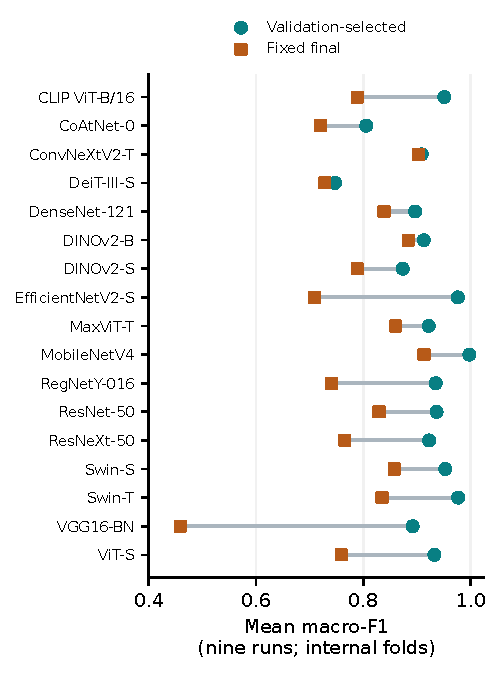
\includegraphics[width=\columnwidth]{endpoints.pdf}
\caption{Validation-selected and fixed-final macro-F1 means for all 17 retained configurations. Each point averages nine runs on the same historical folds; connecting segments highlight endpoint differences and are not uncertainty intervals. Configurations are alphabetical, not performance-ranked.}
\label{fig:endpoints}
\end{figure}


\section{Confidence Diagnostics}\label{app:confidence}
The previously executed confidence analysis averages the saved probabilities from the three explanation-selected architectures and their three seeds within each fold. Each fold's held-out photographs are stratified into three disjoint image subsets for temperature fitting, conformal calibration, and final diagnostics, using the recorded seed $100+\mathrm{fold}$. This subdivision is image-level, not a new tyre-disjoint split. Temperature is fitted by minimising negative log-likelihood on the first subset. Expected calibration error uses 15 equal-width confidence bins. Unlike the standalone ordinal decision in~\eqref{eq:ordinal}, this saved ensemble diagnostic explicitly uses the argmax of its averaged class probabilities.

Conformal nonconformity is $1-p_y$ on the separate calibration subset. The implementation uses the higher empirical quantile at $\min\{1,\lceil(n_{cal}+1)0.9\rceil/n_{cal}\}$ and includes test class $k$ when $1-p_k$ does not exceed that threshold. Coverage and mean set size are then measured on the third subset. The recorded abstention rate counts sets larger than one, leaving empty sets outside that field. We preserve this implementation detail rather than interpreting the field as a complete reject-option metric.


For CORAL outputs $q_0=\sigma(z_0)$ and $q_1=\sigma(z_1)$, the saved implementation constructs $r=(1-q_0,q_0-q_1,q_1)$ and normalises $p_k=\max(r_k,10^{-8})/\sum_j\max(r_j,10^{-8})$. Clamping guarantees a valid probability vector even if cumulative outputs are out of order; it does not guarantee calibrated probabilities. Averaging these vectors and taking argmax can differ from counting thresholds in~\eqref{eq:ordinal}. The uncertainty analysis is consequently a separate decision pipeline, not interchangeable with the reported ordinal classifier.

\subsection{Recorded Outcomes}
Temperature scaling leaves the recorded macro-F1 unchanged and reduces confidence-error metrics on the retained calibration-test subsets (Table~\ref{tab:calibration}). On fold 1, expected calibration error decreases from 0.18955 to 0.07377, and negative log-likelihood from 0.35630 to 0.16226, with 41 test images. Extremely small calibrated errors on the other folds are not evidence of deployment-grade certainty.

At nominal 90\% coverage, the observed conformal coverages are 0.86885, 0.97561, and 0.93939 on folds 0, 1, and 2, respectively (Table~\ref{tab:conformal}). Thus only fold 0 is below nominal in these observed subsets. Mean set sizes below one on folds 0 and 2 imply empty sets. The recorded abstention field does not count all empty-set events and cannot be presented as a complete rejection policy. Small subset sizes, dependent acquisition, and reuse of internal evidence constrain generalisation of these diagnostics.
\begin{table}[t]
\caption{Confidence diagnostics on held-out calibration-test subsets. ECE is the recorded expected calibration error; values near zero on internal folds do not imply external reliability.}
\label{tab:calibration}
\centering
\small
\setlength{\tabcolsep}{4pt}
\begin{tabular}{llrrrr}
\toprule
Fold & Scores & $n$ & F1 & ECE & NLL \\
\midrule
0 & Raw & 61 & 1.0000 & 0.2115 & 0.2425 \\
0 & Temp. & 61 & 1.0000 & 0.0000 & 0.0000 \\
1 & Raw & 41 & 0.8030 & 0.1896 & 0.3563 \\
1 & Temp. & 41 & 0.8030 & 0.0738 & 0.1623 \\
2 & Raw & 33 & 1.0000 & 0.1293 & 0.1438 \\
2 & Temp. & 33 & 1.0000 & 0.0000 & 0.0000 \\
\bottomrule
\end{tabular}
\end{table}

\begin{table}[t]
\caption{Prediction-set diagnostics at nominal 90\% coverage. The recorded abstention field does not count every empty-set event.}
\label{tab:conformal}
\centering
\small
\setlength{\tabcolsep}{4pt}
\begin{tabular}{rrrrrr}
\toprule
Fold & $n_{cal}$ & $n_{test}$ & Coverage & Set size & Abstain \\
\midrule
0 & 62 & 61 & 0.8689 & 0.8689 & 0.0000 \\
1 & 43 & 41 & 0.9756 & 1.0976 & 0.0976 \\
2 & 35 & 33 & 0.9394 & 0.9394 & 0.0000 \\
\bottomrule
\end{tabular}
\end{table}



\FloatBarrier
\bibliographystyle{IEEEtran}
\bibliography{references}
\begin{IEEEbiography}[{\includegraphics[width=1in,height=1.25in,clip, keepaspectratio]{sections/a1.jpg}}]{Edara Sreenivasa Reddy} is currently a Professor (HAG) with the School of Computer Science and Engineering, VIT-AP University, Amaravati, India. He has more than 34 years of academic experience and 18 years of research experience. During his academic
career, he has served in several teaching and administrative positions, including Assistant Professor, Associate Professor, Professor, Senior Professor, Principal, Dean, and Vice-Chancellor.

He has published more than 125 Scopus-indexed journal articles, authored 12 books, contributed 12 chapters to edited research volumes, and obtained 12 patents. Under his supervision, 46 Ph.D. scholars and two M.Phil. scholars have completed their degrees. His research interests include artificial intelligence, machine learning, deep learning, generative artificial intelligence, large language models, and quantum computing.

Prof. Reddy is an NVIDIA University Ambassador for
deep learning and an NVIDIA-certified coach for generative artificial intelligence and large language models. He has also completed professional certification in quantum computing from IBM. He received the Best Computer Science Teacher Award from the Indian Society for
Technical Education. He is a Fellow of the Computer Science Research Council, USA, and an Honorary Fellow of the Academy of Science, Technology and Communications. He is a Senior Member of IEEE and a member of the Indian Society for Technical Education.

\end{IEEEbiography}

\begin{IEEEbiography}[{\includegraphics[width=1in,height=1.25in,clip, keepaspectratio]{sections/a2.jpg}}]{Shanmukesh Bonala} is currently pursuing the B.Tech. degree in computer
science and engineering with VIT-AP University,
Amaravati, India. His research interests include artificial intelligence, computer vision, deep learning, model optimization, and energy-efficient artificial intelligence.

He has contributed to research and development projects in artificial intelligence and computer vision and has published research datasets through IEEE DataPort. His work focuses on the development of scalable and reproducible artificial-intelligence systems. He is an IEEE
Student Member.
\end{IEEEbiography}

\EOD
\end{document}
